\documentclass[11pt]{article}
\makeatletter\def\input@path{{../}}\makeatother
\usepackage{preamble}
\renewcommand{\chaptername}{Chapter 8: Machine learning}
\graphicspath{{figures/}}

\begin{document}

\solutionstitlepage{8}{Machine learning}{All numbers and figures are reproduced by \texttt{ch08/code/ch08.R} (base R, splines, BART and causaldata; about 3 minutes, mostly BART).}

\tableofcontents
\clearpage

\section*{Answers at a glance}
\addcontentsline{toc}{section}{Answers at a glance}
\begin{center}
\small
\renewcommand{\arraystretch}{1.25}
\begin{tabular}{>{\bfseries\color{navy}}r p{0.82\linewidth}}\toprule
1  & $\E(\beta\mid Y)=(1-\kappa)Y$; a half-Cauchy $\tau$ gives $\kappa\sim\dist{Beta}(\frac12,\frac12)$: ``keep or kill''.\\
2  & Horseshoe estimates match SSVS (age $0.26$, net use $-0.25$, green $0.29$); treated and health centre shrunk toward 0.\\
3  & WAIC picks $J=4$; clear increasing-then-flat relationship; only 34\% of points inside the band for $f$ (expected); not monotone.\\
4  & Variance grows with temperature and falls with wind; heteroskedastic model wins (WAIC 985 vs 1001).\\
5  & Wind and temperature are important and non-linear; solar radiation matters less and is roughly linear.\\
6  & GAM: interpretable but additive; GP: flexible with uncertainty but $O(n^3)$; deep learning: scalable but data-hungry; BART: strong default but black-box; quantile regression: robust, distribution-free tails but no single model.\\
7  & Results are robust to \texttt{ntree} and \texttt{power}, sensitive to \texttt{k}; tune \texttt{k} by CV.\\
8  & Year and temperature dominate; BART beats MLR (CV RMSE 651 vs 801), both with $\approx94\%$ coverage.\\
9  & Optimal rule: $A=1$ iff $X_2>0.5$; T-learner BART matches it for 76\% of subjects (S-learner 50\%).\\
10 & Black legislators slightly more likely to reply; MATE $\approx+0.05$ $(-0.05,\ 0.16)$: no clear effect.\\
11 & Equation learning recovers $\beta\approx0.43$, $\gamma\approx0.27$, $R_0\approx1.56$ (truth 0.40, 0.25, 1.60) but its intervals are over-confident.\\\bottomrule
\end{tabular}
\end{center}
\clearpage

% ================================================================= primer
\section*{A five-minute primer on the tools of this chapter}
\addcontentsline{toc}{section}{Primer: the tools of this chapter}

\begin{recall}
\textbf{1. Shrinkage priors.} The \emph{horseshoe} prior $\beta_j\mid\lambda_j,\tau\sim\dist N(0,\lambda_j^2\tau^2)$, $\lambda_j,\tau\sim\text{half-Cauchy}(1)$ shrinks small coefficients strongly toward 0 but leaves large ones almost untouched. A convenient Gibbs representation uses auxiliary inverse-gamma variables: $\lambda_j^2\mid\nu_j\sim\dist{IG}(\frac12,1/\nu_j)$, $\nu_j\sim\dist{IG}(\frac12,1)$ (and similarly for $\tau^2$).

\medskip
\textbf{2. Basis expansions.} Splines write an unknown curve as $f(x)=\sum_jB_j(x)\beta_j$: a non-linear fit by \emph{linear} regression. Additive models (GAMs) add one such curve per covariate.

\medskip
\textbf{3. Heteroskedastic regression.} Model the variance too: $\V(Y_i)=\exp(\mathbf X_i\bm\alpha)$, so $e^{\alpha_j}$ is the multiplicative change in the variance per unit of $X_j$.

\medskip
\textbf{4. BART.} $Y=\sum_{m=1}^{M}g(\mathbf X;T_m,\mathbf M_m)+\varepsilon$: a sum of $M$ (\texttt{ntree}) small regression trees, each kept small by a prior. Tuning: \texttt{ntree} (number of trees), \texttt{power}/\texttt{base} (prior probability that a node at depth $d$ splits, $\text{base}\,(1+d)^{-\text{power}}$), and \texttt{k} (the leaf values are shrunk so that $\pm k$ prior SDs cover the range of $Y$; bigger $k$ = smoother fit).

\medskip
\textbf{5. Causal effects.} With treatment $A$ and confounders $\mathbf X$: $g_a(\mathbf X)=\E(Y\mid A=a,\mathbf X)$; conditional effect $g_1-g_0$; \emph{mixed} (sample-average) treatment effect $\text{MATE}=\frac1n\sum_i\{g_1(\mathbf X_i)-g_0(\mathbf X_i)\}$. A causal interpretation needs no unmeasured confounding, positivity and consistency.
\end{recall}

\clearpage

% ================================================================= Exercise 1
\exercise{8.1 --- Why the horseshoe is a good shrinkage prior}

\begin{problem}{1}
Say $Y|\beta\sim\dist{Normal}(\beta,\sigma^2)$ and $\beta\sim\dist{Normal}(0,\tau^2\sigma^2)$.
\begin{enumerate}[(a)]
\item Prove that the posterior mean of $\beta$ is $\E(\beta|Y)=\{1-\kappa(\tau)\}Y$ for $\kappa(\tau)=1/(1+\tau^2)$.
\item Discuss how small and large $\tau$ lead to different degrees of shrinkage.
\item Prove that if $\tau\sim\text{HC}(1)$ (as in the horseshoe prior), then $\kappa(\tau)\sim\dist{Beta}(1/2,1/2)$.
\item Argue that $\kappa(\tau)\sim\dist{Beta}(1/2,1/2)$ is a reasonable shrinkage prior.
\end{enumerate}
\end{problem}

\begin{restate}
For one noisy observation of a coefficient, show that the posterior mean shrinks the data by a factor $\kappa$, and that the horseshoe's half-Cauchy prior makes $\kappa$ follow a U-shaped distribution.
\end{restate}

\begin{recall}
\begin{itemize}
\item Normal--normal: precisions add; posterior mean = precision-weighted average (Chapter 2 primer).
\item Half-Cauchy(1) density: $f(\tau)=\frac{2}{\pi(1+\tau^2)}$, $\tau>0$.
\item Change of variables: $f_\kappa(\kappa)=f_\tau(\tau(\kappa))\,\big|\frac{\dd\tau}{\dd\kappa}\big|$.
\end{itemize}
\end{recall}

\begin{keyidea}
$\kappa$ is the fraction of the observation that is ``shrunk away'': $\kappa=0$ means no shrinkage, $\kappa=1$ means the estimate is set to 0.
\end{keyidea}

\solution
\step{(a) Posterior mean.}
Likelihood precision $\frac1{\sigma^2}$; prior precision $\frac1{\tau^2\sigma^2}$; prior mean 0. So
\[
\E(\beta\mid Y)=\frac{Y/\sigma^2}{1/\sigma^2+1/(\tau^2\sigma^2)}=\frac{Y}{1+1/\tau^2}=\frac{\tau^2}{1+\tau^2}\,Y=\Big(1-\frac1{1+\tau^2}\Big)Y=\{1-\kappa(\tau)\}Y.
\]
\why{Multiply numerator and denominator by $\sigma^2$, then by $\tau^2$: $\frac{1}{1+1/\tau^2}=\frac{\tau^2}{\tau^2+1}$.}

\step{(b) Small vs.\ large $\tau$.} $\tau\to0$: $\kappa\to1$, $\E(\beta\mid Y)\to0$ --- total shrinkage (the prior insists $\beta\approx0$). $\tau\to\infty$: $\kappa\to0$, $\E(\beta\mid Y)\to Y$ --- no shrinkage (the data speak alone). Intermediate $\tau$ gives partial shrinkage, e.g.\ $\tau=1$: $\kappa=\frac12$, halfway.

\step{(c) Distribution of $\kappa$.}
Invert $\kappa=\frac1{1+\tau^2}$: $\tau=\sqrt{\frac{1-\kappa}{\kappa}}$, and
\[
\frac{\dd\tau}{\dd\kappa}=\frac{1}{2}\Big(\frac{1-\kappa}{\kappa}\Big)^{-1/2}\cdot\Big(-\frac1{\kappa^2}\Big)=-\frac{1}{2\kappa^{3/2}(1-\kappa)^{1/2}}.
\]
Also $1+\tau^2=\frac1\kappa$, so $f_\tau(\tau)=\frac{2}{\pi}\kappa$. Hence
\[
f_\kappa(\kappa)=\frac{2\kappa}{\pi}\cdot\frac{1}{2\kappa^{3/2}(1-\kappa)^{1/2}}=\frac{1}{\pi}\kappa^{-1/2}(1-\kappa)^{-1/2},\qquad0<\kappa<1,
\]
which is the $\dist{Beta}(\frac12,\frac12)$ density ($B(\frac12,\frac12)=\pi$).
\begin{sanity}
Simulation: $10^6$ draws of $\tau=|\text{Cauchy}|$ give $\kappa$ with mean 0.4999 (theory 0.5), $\Prob(\kappa<0.1)=0.2051$ (theory 0.2048) and KS distance 0.0008 from $\dist{Beta}(\frac12,\frac12)$. \checkmark
\end{sanity}
\begin{center}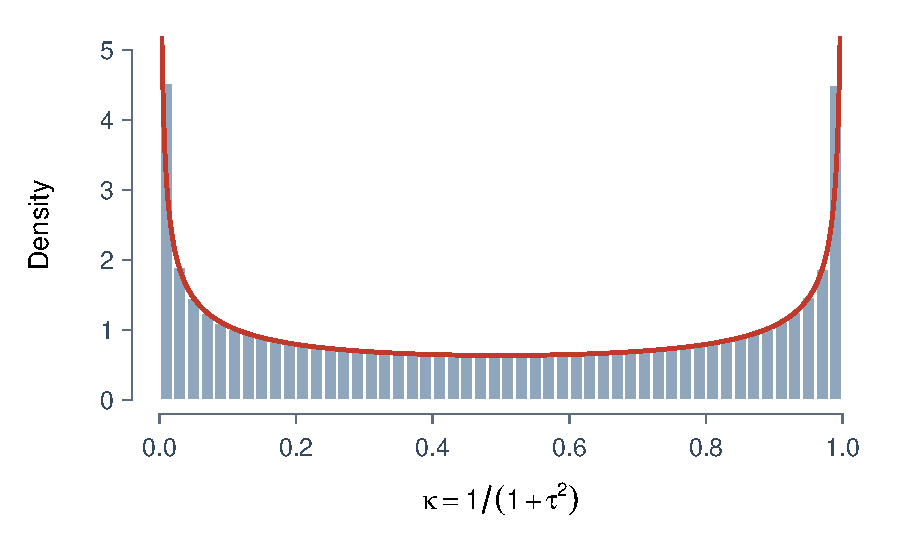
\includegraphics[width=0.62\linewidth]{ex01_kappa.pdf}\end{center}

\step{(d) Why it is a good shrinkage prior.} The $\dist{Beta}(\frac12,\frac12)$ density is U-shaped: most mass is near $\kappa=0$ (\emph{leave the coefficient alone}) and near $\kappa=1$ (\emph{shrink it to zero}). That mimics a spike-and-slab prior --- coefficients are either signal or noise --- but continuously, so it is easy to compute with. Large signals escape shrinkage (the heavy Cauchy tail), while noise is shrunk hard.

\begin{answer}
(a) $\E(\beta\mid Y)=\frac{\tau^2}{1+\tau^2}Y=(1-\kappa)Y$. (b) Small $\tau$: $\kappa\approx1$, heavy shrinkage; large $\tau$: $\kappa\approx0$, none. (c) $f_\kappa(\kappa)=\frac1\pi\kappa^{-1/2}(1-\kappa)^{-1/2}$, i.e.\ $\dist{Beta}(\frac12,\frac12)$. (d) The U shape says ``either keep or kill'', the ideal behaviour for sparse signals.
\end{answer}

\begin{takeaway}
Compare with a $\dist{Uniform}(0,1)$ distribution for $\kappa$, which would favour moderate shrinkage of everything --- bad for sparse problems.
\end{takeaway}

% ================================================================= Exercise 2
\exercise{8.2 --- Horseshoe vs.\ SSVS for the Gambia data}

\begin{problem}{2}
In Section 6.2, we used stochastic search variable selection (SSVS) to analyze childhood malaria data.
\begin{enumerate}[(a)]
\item Fit the model in (6.5) using horseshoe priors for the regression coefficients, and verify MCMC convergence.
\item Compare the results using horseshoe regression with the SSVS results in Table 6.2.
\item In general, what are some pros and cons of SSVS versus horseshoe regression?
\end{enumerate}
\end{problem}

\begin{restate}
Redo the book's malaria variable-selection analysis with a horseshoe prior instead of spike-and-slab and compare.
\end{restate}

\begin{recall}
Model (6.5): $\mathrm{logit}\,\Prob(Y_i=1)=\alpha+\sum_{j=1}^5X_{ij}\beta_j$ with the five covariates (age, net use, treated net, greenness, health centre) standardised. Table 6.2 (SSVS): inclusion probabilities 1.00, 1.00, 1.00, 0.79, 0.56 and medians $0.26,\ -0.25,\ 0.29,\ -0.13,\ -0.05$.
\end{recall}

\begin{keyidea}
Given the local and global scales, the horseshoe is just a normal prior with variances $\lambda_j^2\tau^2$; the scales themselves have inverse-gamma full conditionals (primer, point 1). Only $\bm\beta$ needs a Metropolis step.
\end{keyidea}

\solution
\step{(a) Sampler and convergence.} Each iteration: block Metropolis for $(\alpha,\bm\beta)$ given the scales (acceptance 25\%), then Gibbs updates of $\lambda_j^2,\nu_j,\tau^2,\xi$. Three chains $\times$ 20{,}000 kept draws: all $\hat R\le1.001$, ESS 2{,}150--2{,}670.
\step{(b) Comparison.}
\begin{center}
\small
\begin{tabular}{lccc|cc}\toprule
 & \multicolumn{3}{c|}{Horseshoe} & \multicolumn{2}{c}{SSVS (Table 6.2)}\\
 & median & 95\% interval & GLM (no prior) & incl.\ prob. & median\\\midrule
age & 0.262 & (0.166, 0.361) & 0.273 & 1.00 & 0.26\\
net use & $-0.249$ & $(-0.355,-0.148)$ & $-0.253$ & 1.00 & $-0.25$\\
treated & $-0.122$ & $(-0.241,-0.001)$ & $-0.129$ & 0.79 & $-0.13$\\
greenness & 0.286 & (0.188, 0.388) & 0.294 & 1.00 & 0.29\\
health centre & $-0.085$ & $(-0.193,\ 0.009)$ & $-0.099$ & 0.56 & $-0.05$\\\bottomrule
\end{tabular}
\end{center}
\begin{center}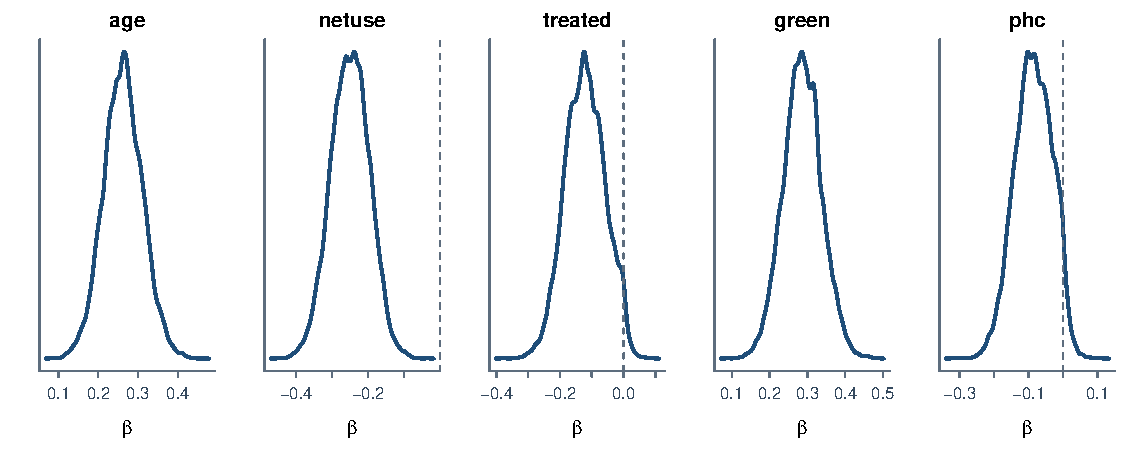
\includegraphics[width=0.98\linewidth]{ex02_horseshoe.pdf}\end{center}
The three strong effects agree almost exactly. For the two weak ones, both methods shrink toward 0: SSVS pushes the health-centre median to $-0.05$ (because 44\% of its posterior mass is exactly 0), the horseshoe to $-0.085$ (continuous shrinkage; its interval just includes 0). Treated nets: both give about $-0.12$ with an interval touching 0.

\step{(c) Pros and cons.}
\begin{itemize}
\item \textbf{SSVS} --- pros: gives inclusion probabilities and model probabilities directly; exact zeros make selection explicit. Cons: discrete indicators mix slowly, especially with correlated predictors (Exercise 6.4); results depend on the slab variance; $2^p$ model space.
\item \textbf{Horseshoe} --- pros: continuous, so standard (or HMC) samplers work and scale to thousands of predictors; few tuning choices; large effects are nearly unbiased. Cons: no exact zeros, so a selection rule must be added (e.g.\ intervals or $\kappa_j$ thresholds); heavy-tailed scales can make sampling slow.
\end{itemize}

\begin{answer}
(a) Converged ($\hat R\le1.001$, ESS $>2{,}000$). (b) Practically identical conclusions: age, net use and greenness are clearly important; treated nets and health centre are weak and shrunk toward 0 by both priors. (c) SSVS gives explicit selection probabilities but mixes poorly in large/correlated problems; the horseshoe scales well and is easy to sample but needs a separate selection rule.
\end{answer}

\begin{takeaway}
For five well-separated predictors the choice hardly matters; the differences appear with many, correlated predictors.
\end{takeaway}

% ================================================================= Exercise 3
\exercise{8.3 --- A spline curve for ozone vs.\ solar radiation}

\begin{problem}{3}
Download the airquality dataset in R. Fit the model
\[
\text{ozone}_i\sim\dist{Normal}\{f(\text{solar.R}_i),\sigma^2\}
\]
where the function $f$ is approximated using spline basis functions.
\begin{enumerate}[(a)]
\item Use model selection tools to select the number of spline basis functions.
\item Make a scatterplot of solar radiation (x-axis) versus ozone (y-axis) and overlay the fitted curve $f$ with a 95\% interval for $f$ for each value of solar radiation. Visually, does the estimated curve fit the data well? Can you conclude that there is a statistically significant relationship between these two variables?
\item Do 95\% of the observations fall in the 95\% credible interval in part (b)? Is this a concern? If not, why? If so, how would you address this concern?
\item Looking at the data, does it appear that $f$ is monotonically increasing? How would you modify your analysis to incorporate the restriction that $f$ is a strictly increasing function of solar radiation?
\end{enumerate}
\end{problem}

\begin{restate}
Fit a smooth curve of ozone against solar radiation, choose its flexibility, check the uncertainty band, and think about forcing the curve to increase.
\end{restate}

\begin{recall}
B-spline regression (Exercise 4.10) and WAIC (Chapter 6). A \emph{credible band for $f$} describes uncertainty about the \emph{mean}; a \emph{prediction interval} also includes the noise $\sigma$.
\end{recall}

\begin{keyidea}
Choose $J$ by WAIC/DIC, then read the band for $f$ and the prediction intervals separately.
\end{keyidea}

\solution
\step{(a) Selecting $J$} (111 days; cubic B-splines with $J$ basis functions; vague priors):
\begin{center}
\begin{tabular}{c|ccccccccc}\toprule
$J$ & 4 & 5 & 6 & 7 & 8 & 9 & 10 & 11 & 12\\\midrule
WAIC & \textbf{1069.9} & 1071.4 & 1073.5 & 1073.5 & 1076.4 & 1076.5 & 1077.0 & 1079.3 & 1082.0\\
DIC & \textbf{1070.6} & 1072.1 & 1074.4 & 1074.6 & 1077.2 & 1077.2 & 1078.0 & 1080.0 & 1082.6\\\bottomrule
\end{tabular}
\end{center}
Both choose $J=4$ (a single cubic polynomial piece) --- the data do not support a wiggly curve.
\step{(b) Fitted curve.}
\begin{center}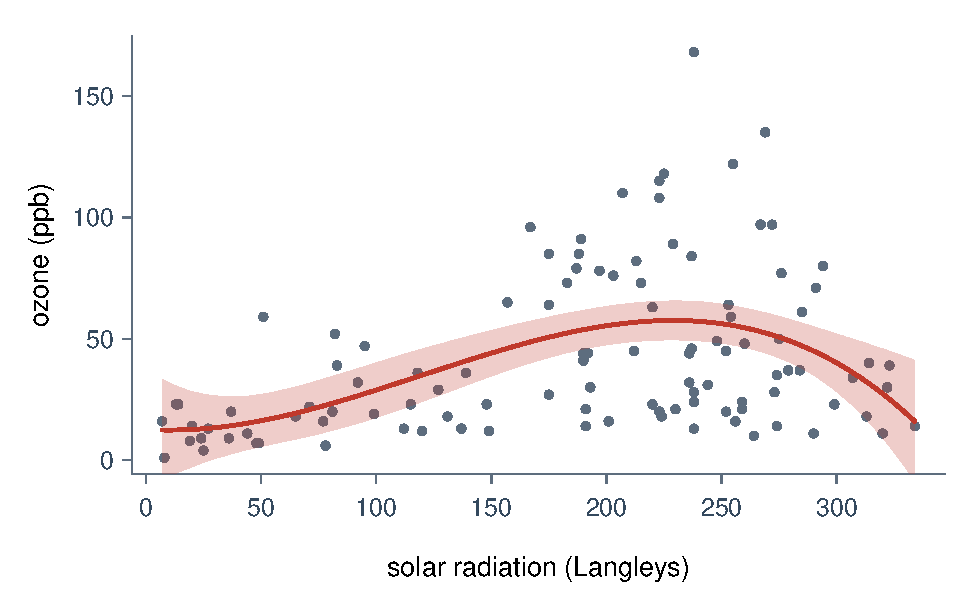
\includegraphics[width=0.72\linewidth]{ex03_spline.pdf}\end{center}
Ozone rises with solar radiation up to about 200--250 Langleys and then levels off or dips. The curve captures the average trend, but the scatter around it is huge. The relationship is clearly real: the posterior of the curve's range $\max f-\min f$ is 51 ppb (95\% CI 34--72), and a linear slope is $11.6$ ppb per SD (95\% CI 5.6--17.8), well away from 0.
\step{(c) Coverage.} Only \textbf{34\%} of observations lie inside the 95\% band for $f$ --- \emph{not} a concern, because that band is for the \emph{mean} ozone at each radiation level, not for individual days. The 95\% \emph{prediction} intervals ($f+$ noise) contain \textbf{96\%} of the observations, as they should. (The real concern is the shape of the noise: it is skewed and grows with the mean, see Exercises 6.2 and 8.4.)
\step{(d) Monotone?} Not quite: the curve dips at high radiation ($\Prob(f\text{ increasing everywhere}\mid\text{data})=0.001$), but the dip is within the noise. To force monotonicity: with B-splines, $f$ is non-decreasing whenever the coefficients are ordered, $\beta_1\le\beta_2\le\dots\le\beta_J$. Reparameterise $\beta_1=\eta_1$, $\beta_j=\beta_{j-1}+e^{\eta_j}$ (positive increments) and put priors on the $\eta_j$; or use a truncated-normal prior restricted to ordered coefficients.

\begin{answer}
(a) WAIC and DIC both select $J=4$. (b) The curve increases then flattens; the relationship is clearly significant (range 34--72 ppb). (c) Only 34\% of points are inside the band for $f$ --- expected, since it is a band for the mean; 96\% are inside the prediction intervals. (d) The estimate is not monotone at the top end; impose monotonicity through ordered B-spline coefficients (positive increments).
\end{answer}

\begin{takeaway}
Never judge a credible band for a mean function by how many data points it contains --- that is the job of prediction intervals.
\end{takeaway}

% ================================================================= Exercise 4
\exercise{8.4 --- A heteroskedastic model for ozone}

\begin{problem}{4}
Using the airquality data from the previous question with response ozone and solar radiation, wind speed and temperature as the covariates, fit the heteroskedastic linear model
\[
Y_i|\bm\beta,\bm\alpha\sim\dist{Normal}\Big\{\sum_{j=1}^pX_{ij}\beta_j,\ \exp\Big(\sum_{j=1}^pX_{ij}\alpha_j\Big)\Big\}.
\]
\begin{enumerate}[(a)]
\item Confirm that the MCMC chains have converged.
\item Summarize the covariate effects on the mean and variance.
\item Does the heteroskedastic fit better than the usual model with constant variance?
\end{enumerate}
\end{problem}

\begin{restate}
Let both the mean ozone and the \emph{spread} of ozone depend on solar radiation, wind and temperature.
\end{restate}

\begin{recall}
Given $\bm\alpha$, the model is weighted least squares with weights $w_i=e^{-\mathbf X_i\bm\alpha}$, so $\bm\beta\mid\bm\alpha$ is normal: precision $\mathbf X^\top\mathbf W\mathbf X+\mathbf I/c^2$. $\bm\alpha$ has no conjugate form (Metropolis).
\end{recall}

\begin{keyidea}
Metropolis-within-Gibbs: exact draw of $\bm\beta$ given $\bm\alpha$; block random walk for $\bm\alpha$ with proposal covariance $\propto2(\mathbf X^\top\mathbf X)^{-1}$ (the large-sample variance of a log-variance regression).
\end{keyidea}

\solution
\step{(a) Convergence.} Three chains $\times$ 20{,}000 kept draws; acceptance for $\bm\alpha$ 28\%; all $\hat R\le1.002$; ESS 1{,}870--8{,}580.
\step{(b) Effects} (covariates standardised):
\begin{center}
\small
\begin{tabular}{lcc|cc}\toprule
 & \multicolumn{2}{c|}{Mean ($\beta$, ppb per SD)} & \multicolumn{2}{c}{Log variance ($\alpha$, per SD)}\\
 & mean & 95\% CI & mean & 95\% CI\\\midrule
intercept & 34.7 & (29.5, 40.6) & 5.92 & (5.66, 6.21)\\
Solar.R & 3.3 & (0.4, 6.4) & 0.20 & $(-0.17,\ 0.55)$\\
Wind & $-2.7$ & $(-6.4,\ 0.1)$ & $\mathbf{-0.64}$ & $(-0.92,-0.36)$\\
Temp & \textbf{9.6} & (5.5, 14.4) & \textbf{0.54} & (0.08, 0.94)\\\bottomrule
\end{tabular}
\end{center}
\why{$e^{0.54}=1.7$: one SD warmer multiplies the variance by 1.7 (SD by 1.3); $e^{-0.64}=0.53$: one SD windier roughly halves the variance.}
Hot, still days have both higher and \emph{more variable} ozone. Once the variance is modelled, the mean effects are smaller than in the constant-variance fit (Exercise 6.1: temperature 15.8, wind $-11.8$), because the few very high-ozone hot days no longer dominate the fit.
\step{(c) Comparison.}
\begin{center}
\begin{tabular}{lccc}\toprule
 & lppd & $p_W$ & WAIC\\\midrule
heteroskedastic & $-481.8$ & 10.7 & \textbf{985.0}\\
constant variance & $-493.8$ & 6.9 & 1001.4\\\bottomrule
\end{tabular}
\end{center}

\begin{answer}
(a) Converged ($\hat R\le1.002$). (b) Temperature raises the mean (+9.6 ppb/SD) and the variance (×1.7/SD); wind lowers the variance (×0.53/SD) and probably the mean; solar radiation has a small positive mean effect and no clear variance effect. (c) Yes: WAIC 985 vs.\ 1001 (difference 16), a substantial improvement.
\end{answer}

\begin{takeaway}
Heteroskedasticity is common whenever a positive response has a wide range; modelling it changes not just the intervals but also the mean estimates.
\end{takeaway}

% ================================================================= Exercise 5
\exercise{8.5 --- An additive model for ozone}

\begin{problem}{5}
Using the airquality data, fit the GAM model
\[
\text{ozone}_i=f_1(\text{solor.R}_i)+f_2(\text{wind.speed}_i)+f_3(\text{temp}_i)+\varepsilon_i
\]
where $\varepsilon_i\iid\dist{Normal}(0,\sigma^2)$ and $f_1$, $f_2$ and $f_3$ are each modeled using B-spline basis expansions with five knots. Which are important predictors of ozone, and which appear to have non-linear effects?
\end{problem}

\begin{restate}
Let each covariate have its own smooth curve, then decide which curves matter and which are genuinely curved.
\end{restate}

\begin{recall}
GAM: $f_k(x)=\sum_jB_{kj}(x)\beta_{kj}$. Each basis is centred so that the intercept is identifiable. Compare models by WAIC: drop a variable to test \emph{importance}; replace its curve with a straight line to test \emph{non-linearity}.
\end{recall}

\begin{keyidea}
Cubic B-splines with 5 interior knots (at the sextiles of each covariate): 8 basis functions per covariate, fitted jointly by the Gibbs sampler for linear regression.
\end{keyidea}

\solution
\step{Fitted curves} (posterior median and 95\% band):
\begin{center}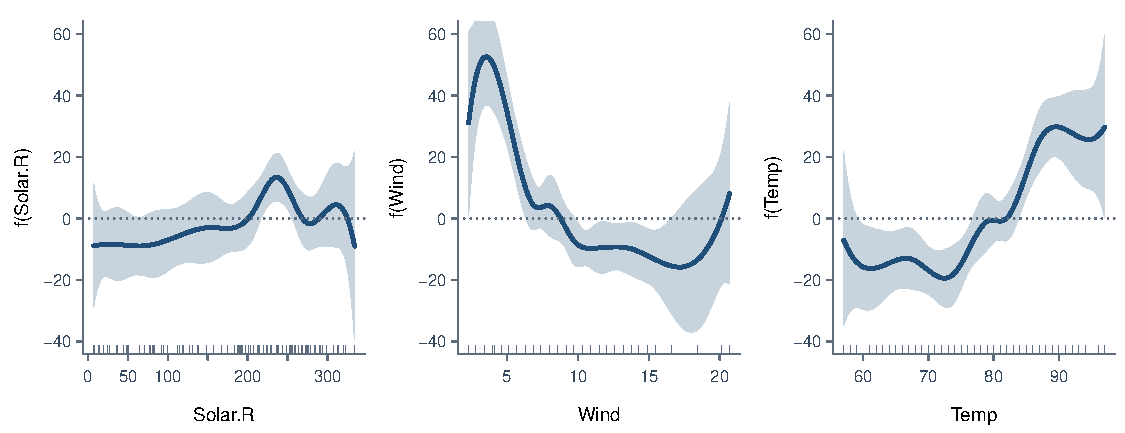
\includegraphics[width=0.98\linewidth]{ex05_gam.pdf}\end{center}
Ozone falls steeply as wind increases from 2 to about 10 mph, then levels off; it rises sharply above about 80$^\circ$F; solar radiation has a gentler, roughly linear positive effect.
\step{Model comparison by WAIC.}
\begin{center}
\begin{tabular}{lcc}\toprule
Model & WAIC & difference from full GAM\\\midrule
full GAM (all smooth) & 978.0 & 0\\\midrule
Solar.R linear, others smooth & \textbf{974.2} & $-3.8$\\
Wind linear, others smooth & 998.1 & $+20.1$\\
Temp linear, others smooth & 984.0 & $+6.1$\\\midrule
without Solar.R & 981.1 & $+3.2$\\
without Wind & 1017.4 & $+39.4$\\
without Temp & 1015.0 & $+37.1$\\\midrule
fully linear model & 1001.3 & $+23.3$\\\bottomrule
\end{tabular}
\end{center}
\why{A large \emph{increase} in WAIC when a curve is made linear means the curvature mattered; a large increase when a variable is dropped means the variable mattered.}

\begin{answer}
\textbf{Important}: wind and temperature (dropping either costs $\approx38$ WAIC units); solar radiation matters much less (dropping it costs 3). \textbf{Non-linear}: wind (making it linear costs 20) and temperature (costs 6); solar radiation's effect is adequately linear (a linear term is even slightly better, $-3.8$). The additive model beats the linear model by 23 WAIC units.
\end{answer}

\begin{takeaway}
A good default is ``smooth everything, then test which smooths can be simplified''.
\end{takeaway}

% ================================================================= Exercise 6
\exercise{8.6 --- Strengths and weaknesses of five ML approaches}

\begin{problem}{6}
Given a strength and a weakness for each of the following approaches:
\begin{enumerate}[(a)]
\item Generalized additive modeling
\item Gaussian process regression
\item Deep learning
\item Bayesian additive regression trees
\item Quantile regression
\end{enumerate}
\end{problem}

\begin{restate}
For five modern regression tools, name one thing each does well and one thing it does badly.
\end{restate}

\begin{keyidea}
Consider interpretability, flexibility (non-linearity and interactions), uncertainty quantification and computational cost.
\end{keyidea}

\solution
\begin{center}
\small
\renewcommand{\arraystretch}{1.35}
\begin{tabular}{p{0.2\linewidth}p{0.36\linewidth}p{0.36\linewidth}}\toprule
Approach & Strength & Weakness\\\midrule
(a) GAM & Interpretable: one smooth curve per covariate that can be plotted; fast (linear in the basis coefficients). & Additive: misses interactions unless they are added by hand; knot choice matters.\\
(b) Gaussian process regression & Very flexible and gives honest, smooth uncertainty bands, especially for interpolation. & Cost grows like $n^3$ (matrix inversion); kernel choice and high dimensions are hard.\\
(c) Deep learning & Learns complex features and interactions from huge, high-dimensional data (images, text); scales with GPUs. & Data-hungry and a black box; full Bayesian uncertainty is expensive or approximate.\\
(d) BART & Excellent default: captures non-linearity and interactions automatically, with uncertainty, and needs little tuning. & Less interpretable; piecewise-constant fits; extrapolates poorly; slower than single-tree methods.\\
(e) Quantile regression & Describes the whole conditional distribution (e.g.\ extremes), robust to outliers, no normality assumption. & Each quantile is a separate model (quantiles can cross); a likelihood (e.g.\ asymmetric Laplace) is needed for a Bayesian version and its uncertainty can be miscalibrated.\\\bottomrule
\end{tabular}
\end{center}

\begin{answer}
See the table.
\end{answer}

\begin{takeaway}
No method is best everywhere: choose by data size, need for interpretation, and whether uncertainty quantification matters.
\end{takeaway}

% ================================================================= Exercise 7
\exercise{8.7 --- BART tuning parameters for the motorcycle data}

\begin{problem}{7}
Fit a semiparametric model to the mcycle data from the MASS package with the time since a motorcycle makes impact as the only predictor and acceleration as the outcome using the wbart function in the BART package.
\begin{enumerate}[(a)]
\item Describe the role of the tuning parameters ntree, power and k.
\item Fit the model and plot the fitted values for several values of these tuning parameters. Are the results sensitive to these tuning parameters? If so, which ones?
\item In practice, how would you select these tuning parameters in a computationally efficient way?
\end{enumerate}
\end{problem}

\begin{restate}
Fit BART to the head-acceleration-after-crash curve, vary its three main tuning knobs, and see which matter.
\end{restate}

\begin{recall}
BART tuning parameters: primer, point 4.
\end{recall}

\begin{keyidea}
Compare settings by their 5-fold cross-validation RMSE, changing one parameter at a time from the defaults (\texttt{ntree}=200, \texttt{power}=2, \texttt{k}=2).
\end{keyidea}

\solution
\step{(a) Roles.}
\begin{itemize}
\item \texttt{ntree}: number of trees in the sum. More trees = each tree does less (smaller leaf effects), a smoother and more stable fit; too few trees can underfit or mix poorly.
\item \texttt{power} (with \texttt{base}): controls how strongly the prior penalises deep trees ($\Prob(\text{split at depth }d)=\text{base}(1+d)^{-\text{power}}$). Larger \texttt{power} = shallower trees = fewer interactions.
\item \texttt{k}: leaf values are given prior SD $\approx\frac{\text{range}(Y)}{2k\sqrt{\texttt{ntree}}}$. Larger \texttt{k} = more shrinkage of the fitted function toward its mean = smoother, less flexible fit.
\end{itemize}
\step{(b) Fits and sensitivity.}
\begin{center}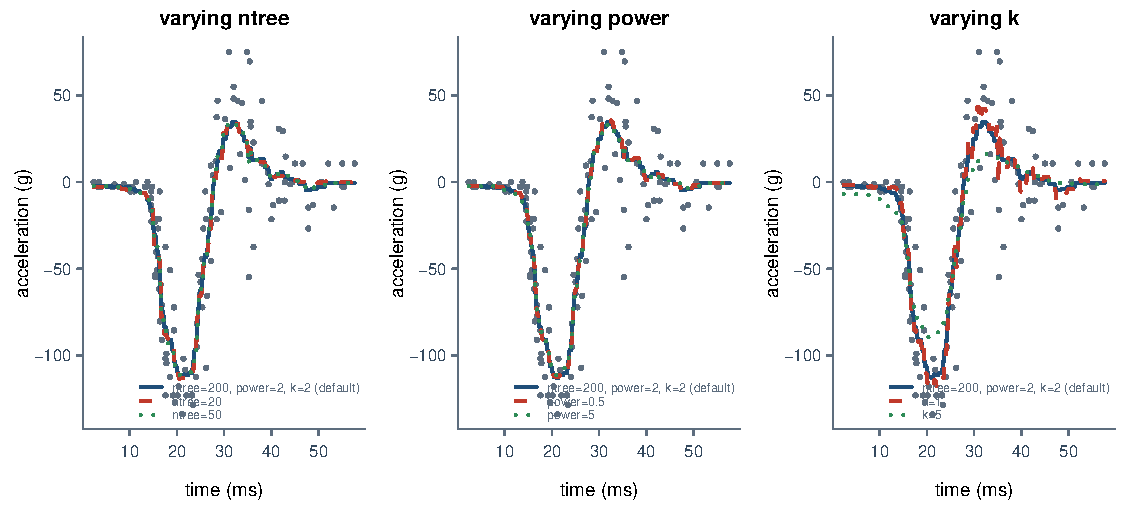
\includegraphics[width=0.98\linewidth]{ex07_bart.pdf}\end{center}
\begin{center}
\begin{tabular}{lcc}\toprule
Setting & 5-fold CV RMSE & posterior mean $\sigma$\\\midrule
default (\texttt{ntree}=200, \texttt{power}=2, \texttt{k}=2) & 24.2 & 22.1\\
\texttt{ntree}=20 & 24.6 & 22.0\\
\texttt{ntree}=50 & 24.6 & 21.9\\
\texttt{power}=0.5 & 24.3 & 22.0\\
\texttt{power}=5 & 24.2 & 22.3\\
\texttt{k}=1 & 25.6 & 21.2\\
\texttt{k}=5 & \textbf{27.2} & 25.1\\\bottomrule
\end{tabular}
\end{center}
The fit is insensitive to \texttt{ntree} and \texttt{power} (CV RMSE within 0.4). It is \emph{sensitive to} \texttt{k}: $k=5$ over-smooths (it cannot follow the sharp dip after 15 ms; RMSE 27.2), and $k=1$ under-smooths (a wigglier fit and slightly worse RMSE).
\step{(c) Efficient selection.} Keep the defaults for \texttt{ntree}/\texttt{power} (robust) and tune \texttt{k} (and possibly the $\sigma$ prior) by $K$-fold CV over a small grid, e.g.\ $k\in\{1,2,3,5\}$, using short chains (a few hundred draws suffice for prediction),, run in parallel (e.g.\ the \texttt{mc.wbart} function in the BART package runs chains on several cores).

\begin{answer}
(a) \texttt{ntree}: number of trees (more = smoother, more stable); \texttt{power}: penalty on tree depth (higher = shallower trees); \texttt{k}: shrinkage of leaf values (higher = smoother function). (b) Results are robust to \texttt{ntree} and \texttt{power} but sensitive to \texttt{k} ($k=5$ clearly over-smooths). (c) Tune mainly \texttt{k} by $K$-fold CV with short, parallel runs.
\end{answer}

\begin{takeaway}
BART's defaults are good; when something needs tuning it is usually the amount of shrinkage (\texttt{k}).
\end{takeaway}

% ================================================================= Exercise 8
\exercise{8.8 --- Daily bike rentals: BART vs.\ linear regression}

\begin{problem}{8}
Download the daily bike sharing data from the book webpage. The response variable is the daily count (cnt) of bike rentals (the first three values are 985, 801 and 1349), which we model as Gaussian.
\begin{enumerate}[(a)]
\item Describe and justify how you process the other variables to be used as predictors.
\item Regress cnt onto the predictors from (a), and determine the most important predictors from your model.
\item Use five-fold cross-validation to compare BART and multiple linear regression in terms of mean squared prediction error and coverage of 95\% prediction intervals.
\end{enumerate}
\end{problem}

\begin{restate}
Predict daily bike rentals in Washington D.C.\ (2011--2012) from calendar and weather variables; compare a linear model with BART.
\end{restate}

\begin{recall}
Categorical variables must be turned into dummy variables for a linear model (one baseline level dropped). Variables that are deterministic functions of others, or of the response, must be removed.
\end{recall}

\begin{keyidea}
Watch out for \textbf{leakage}: \texttt{casual} + \texttt{registered} = \texttt{cnt} exactly, so they must not be predictors.
\end{keyidea}

\solution
\step{(a) Processing.}
\begin{itemize}
\item \textbf{Removed}: \texttt{instant} (row index), \texttt{dteday} (date string, already encoded by \texttt{yr}, \texttt{mnth}, \texttt{weekday}), \texttt{casual} and \texttt{registered} (they add up to the response --- leakage), \texttt{atemp} (``feels-like'' temperature, correlation 0.992 with \texttt{temp}), and \texttt{workingday} (exactly equal to ``weekday and not a holiday'', so perfectly collinear with \texttt{holiday} and the weekday dummies).
\item \textbf{Categorical $\to$ dummies}: \texttt{season} (3 dummies), \texttt{mnth} (11), \texttt{weekday} (6), \texttt{weathersit} (2; the rare category 4 does not occur).
\item \textbf{Kept as numeric}: \texttt{yr} (0/1), \texttt{holiday} (0/1), \texttt{temp}, \texttt{hum}, \texttt{windspeed} (already scaled to $[0,1]$).
\end{itemize}
That gives 27 predictors. For the linear model they are standardised.
\step{(b) Most important predictors.} Linear regression (vague priors), coefficients per SD (rentals per day):
\begin{center}
\small
\begin{tabular}{lcc|lcc}\toprule
Predictor & mean & 95\% CI & Predictor & mean & 95\% CI\\\midrule
year 2012 & 1010 & (953, 1068) & weather 3 (rain/snow) & $-331$ & $(-398,-264)$\\
temperature & 821 & (676, 969) & September & 270 & (125, 415)\\
winter (season 4) & 678 & (528, 828) & wind speed & $-227$ & $(-290,-167)$\\
summer (season 2) & 386 & (229, 539) & weather 2 (mist) & $-220$ & $(-291,-148)$\\
fall (season 3) & 364 & (180, 547) & & & \\\bottomrule
\end{tabular}
\end{center}
BART's variable-inclusion proportions agree: temperature (0.079), year (0.057), bad weather (0.045), season 4 (0.041), humidity, wind speed. So: \textbf{year} (system growth), \textbf{temperature}, \textbf{season} and \textbf{weather} are the main drivers. (Residual SD: 771 for the linear model, 547 for BART.)
\step{(c) 5-fold cross-validation.}
\begin{center}
\begin{tabular}{lccc}\toprule
 & RMSE & MSE & coverage of 95\% PI\\\midrule
linear regression & 801 & $6.41\times10^5$ & 0.938\\
BART & \textbf{651} & $\mathbf{4.23\times10^5}$ & 0.937\\\bottomrule
\end{tabular}
\end{center}

\begin{answer}
(a) Drop identifiers, leakage variables (\texttt{casual}, \texttt{registered}) and redundant ones (\texttt{atemp}, \texttt{workingday}); dummy-code season, month, weekday and weather. (b) Year, temperature, season and weather are the most important predictors. (c) BART reduces the MSE by about 34\% (RMSE 651 vs.\ 801); both have close to nominal (94\%) interval coverage.
\end{answer}

\begin{takeaway}
BART wins because it captures non-linear effects (e.g.\ temperature helps only up to a point) and interactions (weather $\times$ season) automatically.
\end{takeaway}

% ================================================================= Exercise 9
\exercise{8.9 --- Learning an optimal treatment rule}

\begin{problem}{9}
Simulate 100 observations from (8.29) with response $Y$, treatment $A$ and potential confounders $\mathbf X$ using the following R code:
\begin{lstlisting}
set.seed(919)
X  <- matrix(runif(500),100,5)
A  <- rbinom(100,1,X[,1])
g0 <- 2 + cos(10*X[,3])
g1 <- 1 + 2*X[,2] + cos(10*X[,3])
Y  <- rnorm(100,(1-A)*g0+A*g1,1)
\end{lstlisting}
\begin{enumerate}[(a)]
\item Assuming this model is known, what is the optimal decision rule? That is, for an observation with a given value of $\mathbf X$, which value (0 or 1) of $A$ would maximize the fitted mean response? Express the optimal rule as an equation, e.g., $g_1>g_0$ if $X_2>X_3$.
\item Fit a Bayesian machine learning model to these data, and summarize the fitted model.
\item Using the fitted model, for each of the 100 observations in the training data, which value of the treatment maximizes the mean response? For what proportion of the observations does this match the optimal treatment rule from (a)?
\item Give the main assumptions needed to have a casual interpretation of these results.
\end{enumerate}
\end{problem}

\begin{restate}
Treatment helps some subjects and harms others depending on $X_2$. Recover who should be treated from 100 noisy observations.
\end{restate}

\begin{recall}
Causal effects: primer, point 5. \textbf{S-learner}: one model $\hat g(A,\mathbf X)$, effect $\hat g(1,\mathbf X)-\hat g(0,\mathbf X)$. \textbf{T-learner}: separate models $\hat g_1(\mathbf X)$ on treated units and $\hat g_0(\mathbf X)$ on untreated units.
\end{recall}

\begin{keyidea}
The treatment effect is $g_1-g_0=2X_2-1$: it depends only on $X_2$. A model must capture that interaction to find the rule.
\end{keyidea}

\solution
\step{(a) Optimal rule.} $g_1-g_0=(1+2X_2+\cos(10X_3))-(2+\cos(10X_3))=2X_2-1$, so
\[
g_1>g_0\iff X_2>0.5:\qquad\text{treat }(A=1)\text{ if }X_2>0.5,\ \text{otherwise }A=0.
\]
\step{(b) Fitted models.} 49 of the 100 subjects were treated (treatment depends on $X_1$ --- confounding by design).
\begin{itemize}
\item \textbf{S-learner} (one BART with $A$ as an input): fits the outcome surface but shrinks the interaction: estimated effects range only from $-0.29$ to $0.08$, although they correlate 0.84 with the truth.
\item \textbf{T-learner} (two BARTs): effects range from $-1.89$ to $1.61$ (truth $-1$ to $1$), correlation 0.64 with the truth; residual SD $\approx0.90$ in each arm (truth 1). The fitted $g_1,g_0$ correlate 0.50 and 0.64 with the true functions --- with only $\approx50$ noisy points per arm, the $\cos(10X_3)$ wiggle is hard to learn.
\end{itemize}
\begin{center}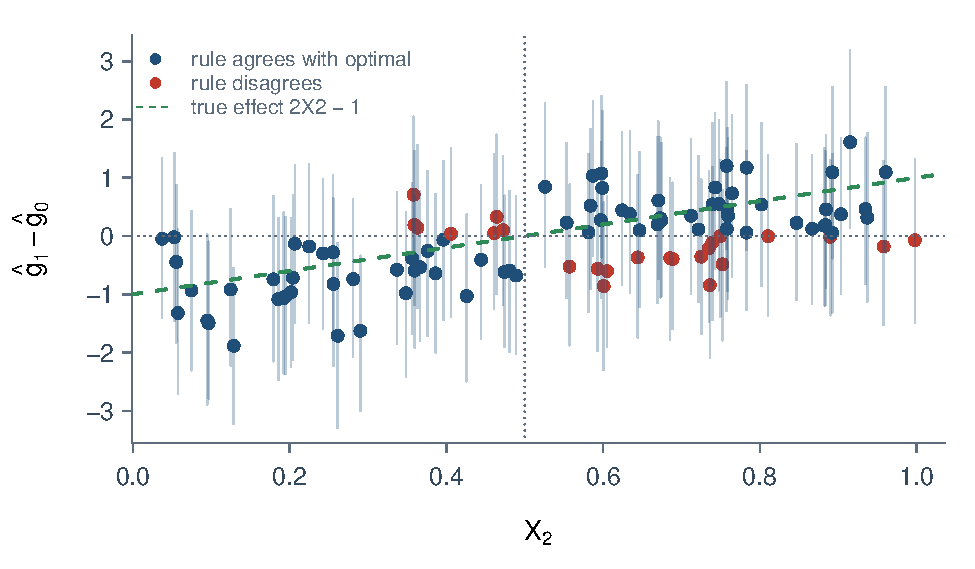
\includegraphics[width=0.72\linewidth]{ex09_cate.pdf}\end{center}
\step{(c) Agreement with the optimal rule.} Treat if the posterior mean of $\hat g_1-\hat g_0$ is positive:
\begin{center}
\begin{tabular}{lc}\toprule
Learner & agreement with ``$X_2>0.5$''\\\midrule
S-learner & 50\%\\
T-learner & \textbf{76\%}\\\bottomrule
\end{tabular}
\end{center}
The S-learner's shrunken effects are nearly all on one side of zero, so its rule is no better than a coin toss even though it ranks subjects well; the T-learner recovers the rule for three quarters of the subjects.
\step{(d) Causal assumptions.}
\begin{itemize}
\item \textbf{No unmeasured confounding}: given $\mathbf X$, treatment assignment is independent of the potential outcomes (true here: $A$ depends only on $X_1$).
\item \textbf{Positivity}: every subject has a non-zero chance of each treatment, $0<\Prob(A=1\mid\mathbf X)<1$ (here $\Prob(A=1\mid\mathbf X)=X_1$, which is near 0 or 1 for some subjects).
\item \textbf{Consistency / SUTVA}: the observed outcome equals the potential outcome under the treatment received, with no interference between subjects.
\item The model must be flexible enough to capture $g_0$ and $g_1$.
\end{itemize}

\begin{answer}
(a) Treat if and only if $X_2>0.5$. (b) BART fits (S- and T-learner); the T-learner captures the effect heterogeneity better. (c) The T-learner's rule matches the optimal rule for 76\% of subjects (S-learner 50\%). (d) No unmeasured confounding, positivity, consistency/no interference, and a correctly flexible model.
\end{answer}

\begin{takeaway}
Ranking subjects by benefit and getting the \emph{sign} right are different tasks; shrinkage priors can hurt the latter. With 100 noisy observations, expect imperfect rules.
\end{takeaway}

% ================================================================= Exercise 10
\exercise{8.10 --- Do black legislators respond more to black constituents?}

\begin{problem}{10}
Load the black\_politicians dataset from the causaldata package. To simplify the problem, we will analyze only data with treat\_out equal to one. The data consist of the results of emails sent to legislators from black voters from outside the legislator's district. The response variable is the binary indicator of whether the legislator responded to the email, responded. The treatment variable is whether the legislator is black, leg\_black, and the remaining 11 variables are used as potential confounders.
\begin{enumerate}[(a)]
\item Perform a Bayesian logistic regression that includes only the treatment variable as a predictor. Summarize the treatment effect. What are some potential sources of bias in this analysis?
\item Perform a Bayesian logistic regression that includes both the treatment variable and the confounders (as linear terms), and summarize the treatment effect. Are the results affected by including the potential confounders?
\item Perform a semiparametric Bayesian logistic regression using the function lbart in the package BART. Compute the posterior distribution of the mixed average treatment effect (MATE), and summarize the results.
\end{enumerate}
\end{problem}

\begin{restate}
Emails from (out-of-district) black voters were sent to state legislators. Did black legislators reply more often than other legislators, and does that survive adjustment for district characteristics?
\end{restate}

\begin{recall}
Logistic regression and block Metropolis (Chapter 4 primer). MATE: primer, point 5, computed draw-by-draw as $\frac1n\sum_i\{\hat p_i(A=1)-\hat p_i(A=0)\}$.
\end{recall}

\begin{keyidea}
Black legislators represent very different districts (far more black residents, more Democratic, more Southern), so the unadjusted comparison mixes the legislator's race with district characteristics.
\end{keyidea}

\solution
\step{Data.} 2{,}779 emails; response rate 31.8\% for black legislators (179 emails) vs.\ 28.7\% for others.
\step{(a) Treatment only.} log OR $0.15$ $(-0.19,\ 0.47)$, OR $1.16$, $\Prob(\text{OR}>1)=0.81$: a small, uncertain positive difference. \emph{Possible biases}: confounding by district demographics (black legislators' districts differ greatly --- standardised mean difference 2.98 for \% black, 0.96 for Democratic party, 0.62 for South), by legislator characteristics (party, chamber, staff resources, professionalism of the legislature), and by email-handling practices.
\step{(b) With the 11 confounders} (standardised linear terms): log OR $0.11$ $(-0.44,\ 0.62)$, OR $1.12$, $\Prob(\text{OR}>1)=0.67$. The point estimate barely moves but the interval widens by $\approx60\%$: the treatment is strongly associated with the confounders, so adjusting removes information. Strong confounder effects: legislature professionalism (Squire index, $+0.21$), senators ($+0.19$), Democrats ($-0.18$), larger districts ($-0.14$).
\step{(c) BART (\texttt{lbart}).} Predict each email's response probability with \texttt{leg\_black} set to 1 and to 0, average the difference over the sample, draw by draw:
\begin{center}
\begin{tabular}{lcc}\toprule
 & MATE (difference in response probability) & 95\% CI\\\midrule
naive difference & 0.032 & ---\\
linear logistic (b) & 0.024 & $(-0.081,\ 0.134)$\\
BART & 0.046 & $(-0.051,\ 0.161)$\\\bottomrule
\end{tabular}
\end{center}
\begin{center}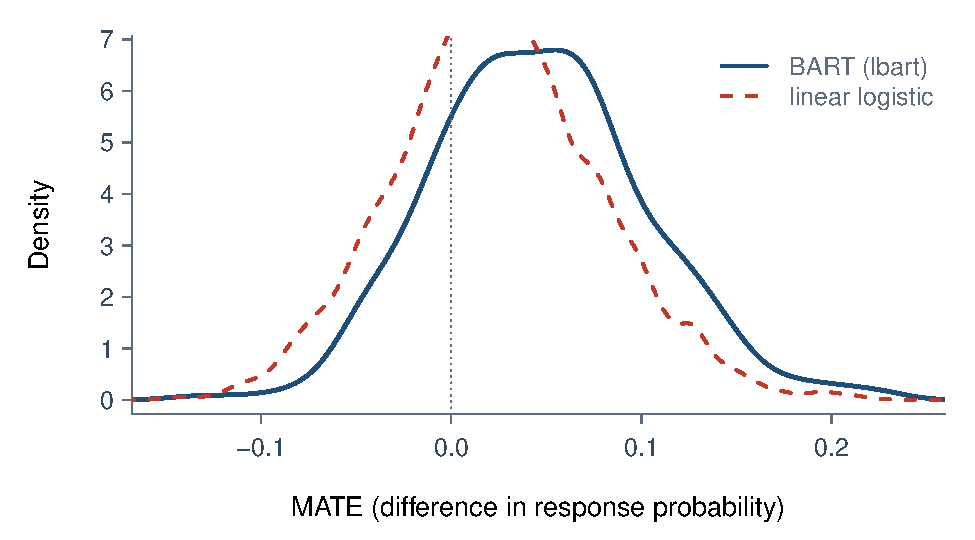
\includegraphics[width=0.66\linewidth]{ex10_mate.pdf}\end{center}
$\Prob(\text{MATE}>0)=0.79$ under BART.

\begin{answer}
(a) OR 1.16 $(0.83,\ 1.60)$: a weak, uncertain advantage for black legislators, potentially biased by large differences in their districts. (b) Adjusting for the confounders leaves the estimate similar (OR 1.12) but much less certain. (c) BART MATE $=+0.05$ (95\% CI $-0.05$ to $0.16$), $\Prob(\text{MATE}>0)=0.79$: black legislators may be somewhat more responsive to out-of-district black constituents, but the data do not establish it.
\end{answer}

\begin{takeaway}
When treated and control groups differ this much on confounders (poor overlap), adjustment widens intervals --- an honest reflection of how little the data can say.
\end{takeaway}

% ================================================================= Exercise 11
\exercise{8.11 --- Equation learning for an SIR epidemic}

\begin{problem}{11}
Use the R package covid19.analytics to generate data from the SIR model similar to (8.6.5) for Uruguay as
\begin{lstlisting}
data <- covid19.data("ts-confirmed")
SIR  <- generate.SIR.model(data,"Uruguay",
          tot.population=3500000)
\end{lstlisting}
Assume that you observe noisy (with multiplicative gamma errors) versions of the number of susceptible and infected,
\begin{lstlisting}
set.seed(1)
S <- SIR$model$S*rgamma(90,100,100)
I <- SIR$model$I*rgamma(90,100,100)
\end{lstlisting}
Fit a Bayesian equation learning model that regresses $dI(t)/dt$ onto $S(t)$ and $I(t)$, and summarize the disease dynamics you learn from the data.
\end{problem}

\begin{note}
\texttt{covid19.analytics} downloads live (and now discontinued) Johns Hopkins data feeds, so its output is not reproducible. We therefore generate the SIR trajectory directly: population $N=3.5$ million, 50 initial infections, transmission rate $\beta=0.40$ and recovery rate $\gamma=0.25$ per day ($R_0=1.6$), 90 days, solved by 4th-order Runge--Kutta. The noise is added exactly as in the exercise (\texttt{set.seed(1)}; $\times\dist{Gamma}(100,100)$, i.e.\ about 10\% multiplicative noise).
\end{note}

\begin{restate}
From noisy daily counts of susceptible and infected people, recover the equation that governs the epidemic, and its transmission and recovery rates.
\end{restate}

\begin{recall}
SIR model: $\frac{\dd S}{\dd t}=-\beta\frac{SI}{N}$, $\frac{\dd I}{\dd t}=\beta\frac{SI}{N}-\gamma I$. Dividing by $I$:
\[
\frac{\dd\log I}{\dd t}=\beta\,\frac SN-\gamma,
\]
which is \emph{linear} in $(\beta,\gamma)$. $R_0=\beta/\gamma$ is the average number of people one infected person infects in a fully susceptible population.
\end{recall}

\begin{keyidea}
Equation learning in two steps: (1) estimate the derivative from the data by smoothing; (2) regress it on a \emph{library} of candidate terms and see which terms are needed. Working with $\log I$ turns the multiplicative noise into additive noise.
\end{keyidea}

\solution
\step{Step 1 --- derivatives.} Smooth $\log I(t)$ and $\log S(t)$ with smoothing splines (smoothness chosen by generalised cross-validation: 8.5 and 6.9 effective degrees of freedom) and differentiate the smooth of $\log I$.
\step{Step 2 --- library regression.} Regress $\frac{\dd\log I}{\dd t}$ on $\{1,\ S/N,\ I/N\}$ (vague priors; response in \% per day so the variance prior is genuinely vague):
\begin{center}
\begin{tabular}{lcc}\toprule
Term & coefficient & 95\% CI\\\midrule
constant ($=-\gamma$) & $-0.272$ & $(-0.279,\ -0.265)$\\
$S/N$ ($=\beta$) & 0.426 & (0.419, 0.433)\\
$I/N$ (not in SIR) & $-0.016$ & $(-0.068,\ 0.034)$\\\bottomrule
\end{tabular}
\end{center}
The extra term $I/N$ is clearly unnecessary (its interval comfortably includes 0): the data ``learn'' the SIR structure.
\step{Step 3 --- reduced model} $\frac{\dd\log I}{\dd t}=\beta\frac SN-\gamma$:
\begin{center}
\begin{tabular}{lccc}\toprule
 & posterior mean & 95\% CI & truth\\\midrule
$\beta$ & 0.428 & (0.423, 0.433) & 0.40\\
$\gamma$ & 0.274 & (0.270, 0.278) & 0.25\\
$R_0=\beta/\gamma$ & 1.561 & (1.553, 1.569) & 1.60\\\bottomrule
\end{tabular}
\end{center}
\begin{center}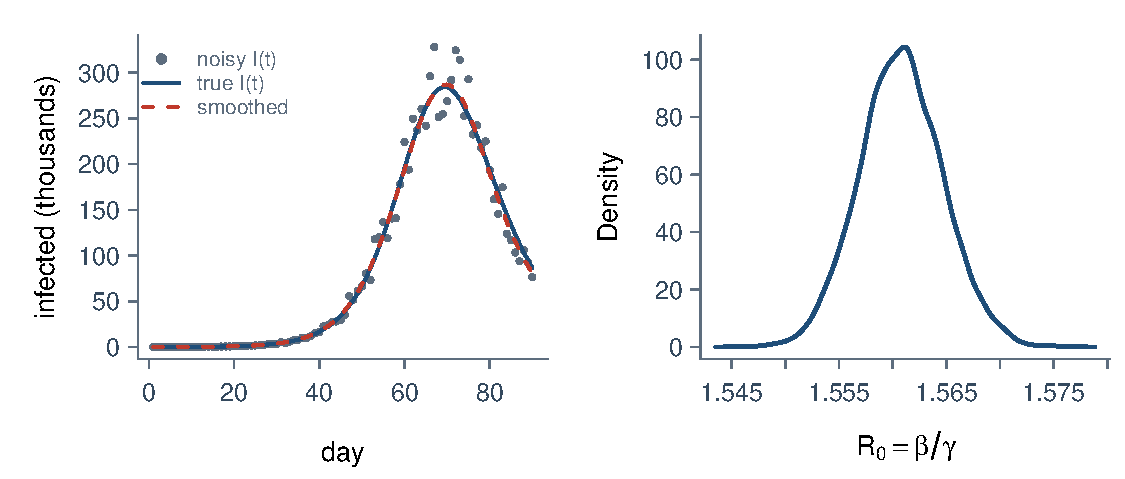
\includegraphics[width=0.98\linewidth]{ex11_sir.pdf}\end{center}
\step{Dynamics learned.} Each infected person infects $\approx0.43$ others per day and recovers after $1/\gamma\approx3.7$ days on average; $R_0\approx1.56>1$, so the epidemic grows until enough people are immune ($S/N<1/R_0\approx0.64$), then declines. Infections peak around day 69 (about 284{,}000 infected) and 60\% of the population has been infected by day 90.

\begin{sanity}
The estimates are close to the truth (all within 10\%), but the 95\% intervals are \emph{too narrow} and do not contain the true $\beta$ and $\gamma$. Two reasons: (i) the regression treats the smoothed derivatives as independent data, although smoothing makes their errors strongly correlated; (ii) early in the epidemic $S/N\approx1$, so $\beta$ and $\gamma$ are nearly confounded (posterior correlation 0.97) and only their difference (the growth rate) and ratio are well determined. A fully Bayesian alternative is to fit the ODE solution directly to the noisy counts (an ODE likelihood), which propagates all uncertainty.
\end{sanity}

\begin{answer}
The learned equation is $\frac{\dd I}{\dd t}\approx0.43\frac{SI}{N}-0.27I$ (an extra $I^2$-type term is not supported): transmission $\beta\approx0.43$/day, recovery $\gamma\approx0.27$/day (infectious period $\approx3.7$ days), $R_0\approx1.56$. Estimates are close to the truth (0.40, 0.25, 1.60), but the two-step method's intervals are over-confident.
\end{answer}

\begin{takeaway}
Equation learning can recover the \emph{form} of the dynamics from noisy data; for honest \emph{uncertainty} about the rates, fit the differential equation itself.
\end{takeaway}

\end{document}
